\documentclass{beamer}
\usepackage{siunitx,booktabs,xcolor,xspace,multirow,graphicx,lipsum}
\usepackage[spanish,mexico,es-noindentfirst]{babel}
\usepackage[utf8]{inputenc}
\usepackage{tikz}
\usepackage{subcaption}
\usepackage[charter]{mathdesign}
\usetheme{Madrid}
\usepackage{tcolorbox}
\usepackage{hyperref}

\usefonttheme{serif}


\setbeamertemplate{frametitle}{
  \begin{beamercolorbox}[wd=\paperwidth,ht=1cm, sep=0.25cm]{frametitle}
    \begin{tikzpicture}[remember picture,overlay]
      \node[anchor=north east] at (current page.north east) {
\includegraphics[height=0.75cm]{special_figures/Turix_nobg.png}};
    \end{tikzpicture}
    \usebeamerfont{frametitle}\bfseries\insertframetitle
  \end{beamercolorbox}
}

\setbeamertemplate{caption}[numbered]
\setbeamercolor{frametitle}{bg=beamer_color,fg=white}
\setbeamercolor{author in head/foot}{bg=beamer_color,fg=white}
\setbeamercolor{title in head/foot}{bg=beamer_color,fg=white}
\setbeamercolor{date in head/foot}{bg=beamer_color,fg=white}
\setbeamercolor{titlelike}{parent=structure,bg=beamer_color,fg=white}
\setbeamertemplate{section in toc}[sections numbered]
\setbeamertemplate{subsection in toc}[subsections numbered]
\setbeamerfont{section in toc}{series=\bfseries}
\setbeamercolor{section in toc}{fg=black}
\setbeamercolor{caption name}{fg=blue}
\setbeamerfont{caption name}{series=\bfseries}
\setbeamerfont{caption}{size=\small}
\setbeamercolor{bibliography entry author}{fg=black}
\setbeamercolor{bibliography entry title}{fg=black} 
\setbeamertemplate{section in toc}{\inserttocsectionnumber.~\inserttocsection\par}
\setbeamertemplate{subsection in toc}{\hspace{1.5em}\inserttocsectionnumber.\inserttocsubsectionnumber~\inserttocsubsection\par}



\title[\textbf{Título de la tesis}]{\textbf{Título de la tesis}}
\author[\textbf{Nombre del tesista}]{\textbf{Nombre del tesista \\ micorreoelectronico@tuxtla.tecnm.mx}}
\date{\textbf{Mes, Año}}

\renewcommand{\maketitle}{
\vspace{0.5\baselineskip}

\begin{center}
    
\includegraphics[height=1.25cm]{special_figures/TecNM.jpg}\hfill
    
\includegraphics[height=1.25cm]{special_figures/ITTG.png}\hfill
    
\includegraphics[height=1.25cm]{special_figures/Turix.png}\hfill
\end{center}

\begin{center}
    \textbf{MAESTRÍA EN CIENCIAS EN INGENERÍA MECATRÓNICA}
\end{center}

\titlepage
\vspace{\baselineskip}
\begin{center}
    \small
    \vspace{-2.5\baselineskip}
    Director(es) de la Tesis: Nombre(s) de director(es) de la tesis\\
    Revisor 1: Nombre del primer revisor\\
    Revisor 2: Nombre del segundo revisor\\
\end{center}
}

% \AtBeginSection[ ]
% {
% \begin{frame}{Contenido de la presentación}
% \tableofcontents[currentsection,subsectionstyle = shaded]
% \end{frame}
% }

% \AtBeginSubsection[ ]
% {
% \begin{frame}{Contenido de la presentación}
% \tableofcontents[currentsection,currentsubsection]
% \end{frame}
% }

% Définir couleur verte
% \definecolor{beamer_color}{RGB}{64, 145, 63}
% \definecolor{backframe_color}{RGB}{228, 242, 232}

% Définir couleur violette
\definecolor{beamer_color}{RGB}{70,2,105}
\definecolor{backframe_color}{RGB}{235, 196, 245}


\begin{document}

\begin{frame}
    \maketitle
\end{frame}

\begin{frame}{Sommaire de la présentation}
    \sommairetimeline{0}
\end{frame}

\section{Contexte général}

\subsection{Présentation de l'entreprise}
\begin{frame}{Présentation de l'entreprise}
    \begin{figure}
        \centering
        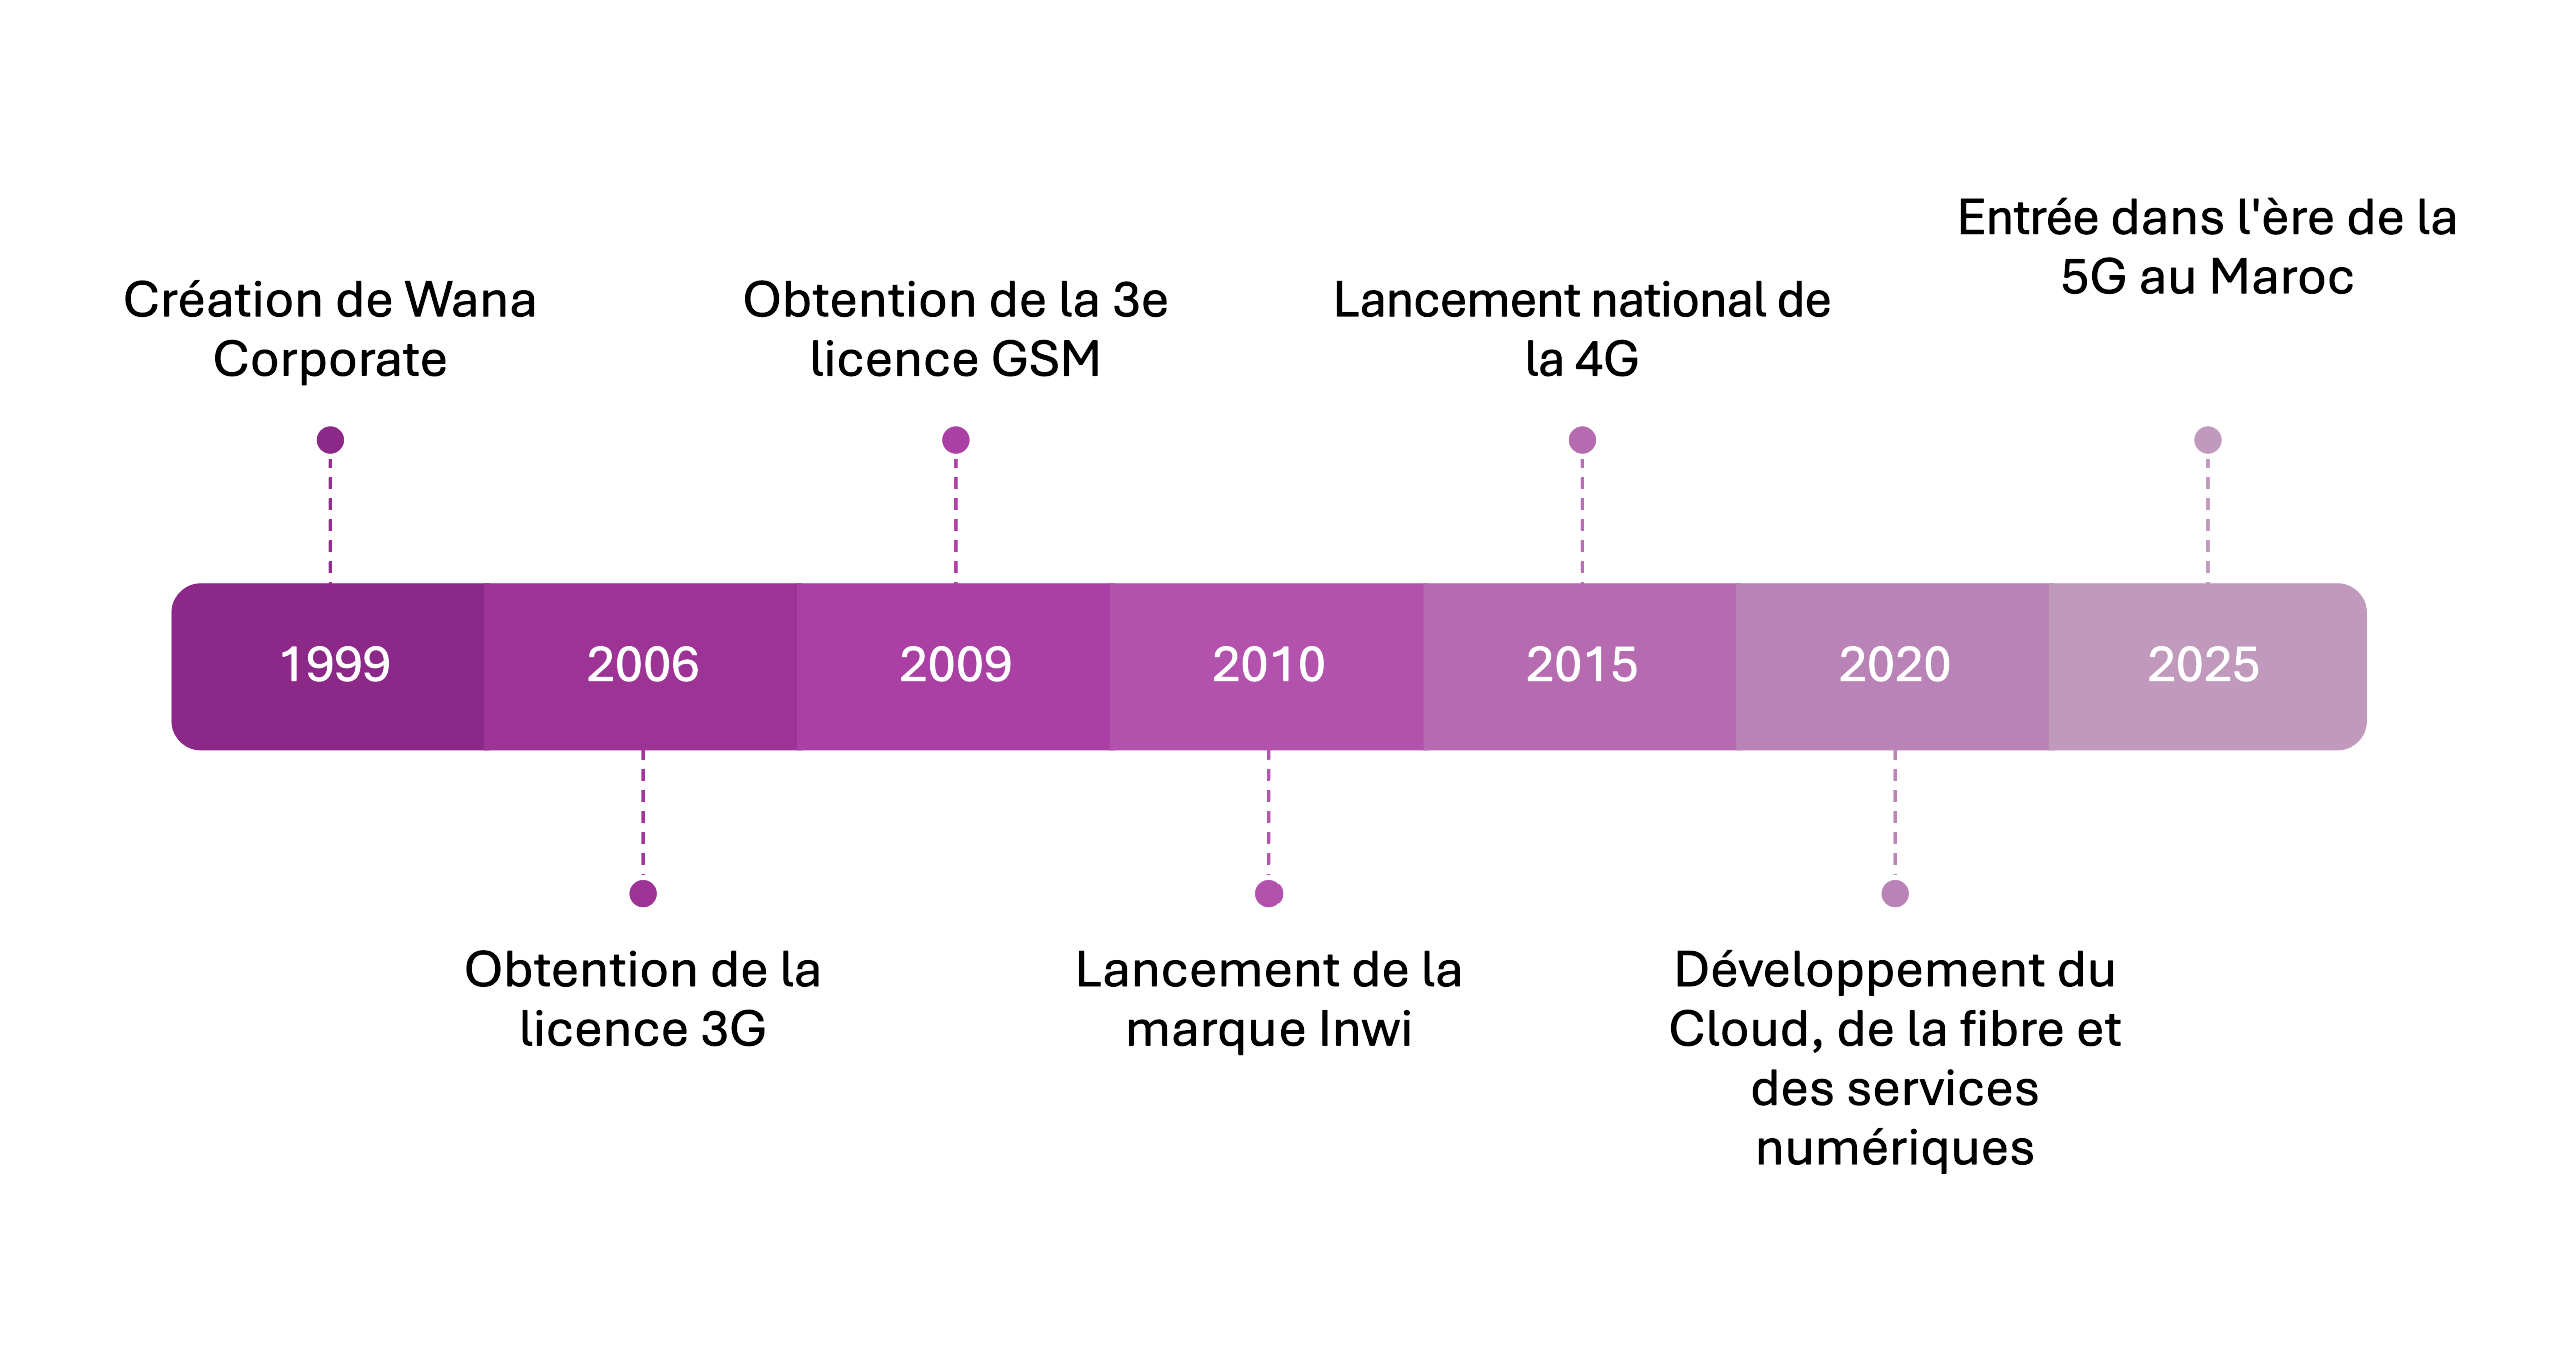
\includegraphics[width=1\linewidth]{chronologie.png}
    \end{figure}
\end{frame}
\begin{frame}{Présentation de l'entreprise}
\begin{figure}
    \centering
    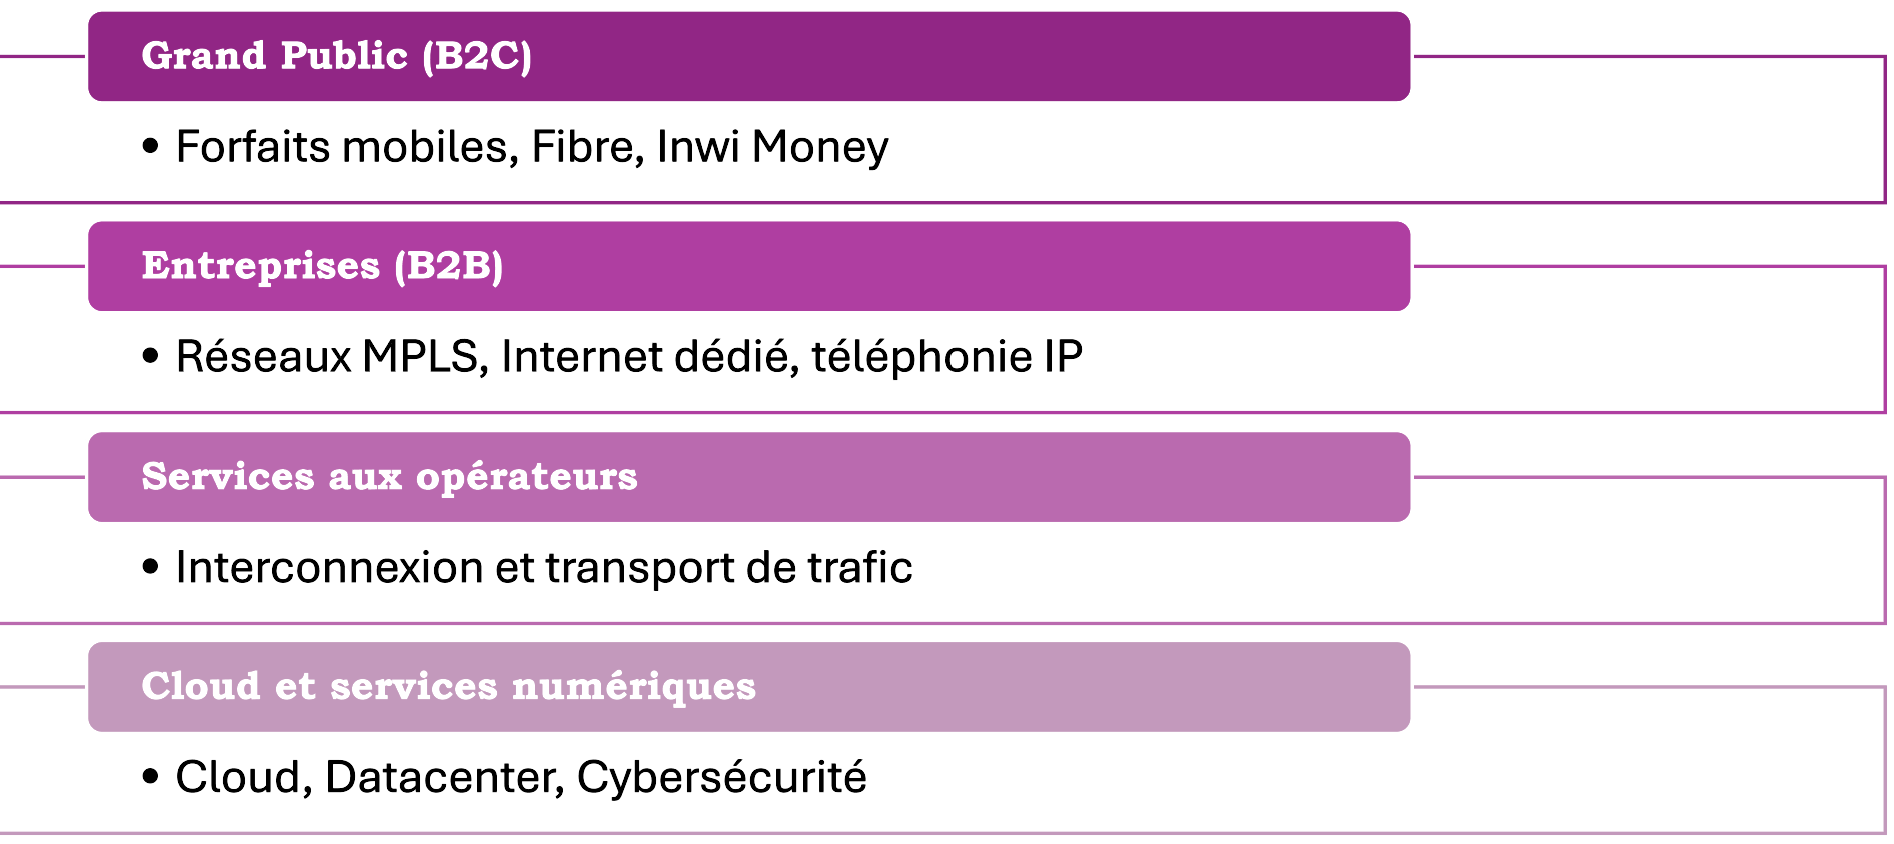
\includegraphics[width=1\linewidth]{activites.png}
\end{figure}
\end{frame}

\subsection{Problématique}
\begin{frame}{Problématique}
\begin{columns}[c]
        \begin{column}{0.32\textwidth}
            \begin{block}{\centering Contexte}
            \scriptsize
            
            \setlength{\itemsep}{3pt}
            \setlength{\parskip}{0pt}
            \setlength{\parsep}{0pt}
            
            \begin{itemize}
                \item[\ding{45}] Flux d'alertes important et dispersé
                \item[\ding{45}] Manque d'automatisation
                \item[\ding{45}] Besoin d'améliorer la productivité des équipes
            \end{itemize}
            
            \end{block}
        \end{column}
        
        \begin{column}{0.33\textwidth}
            \centering
            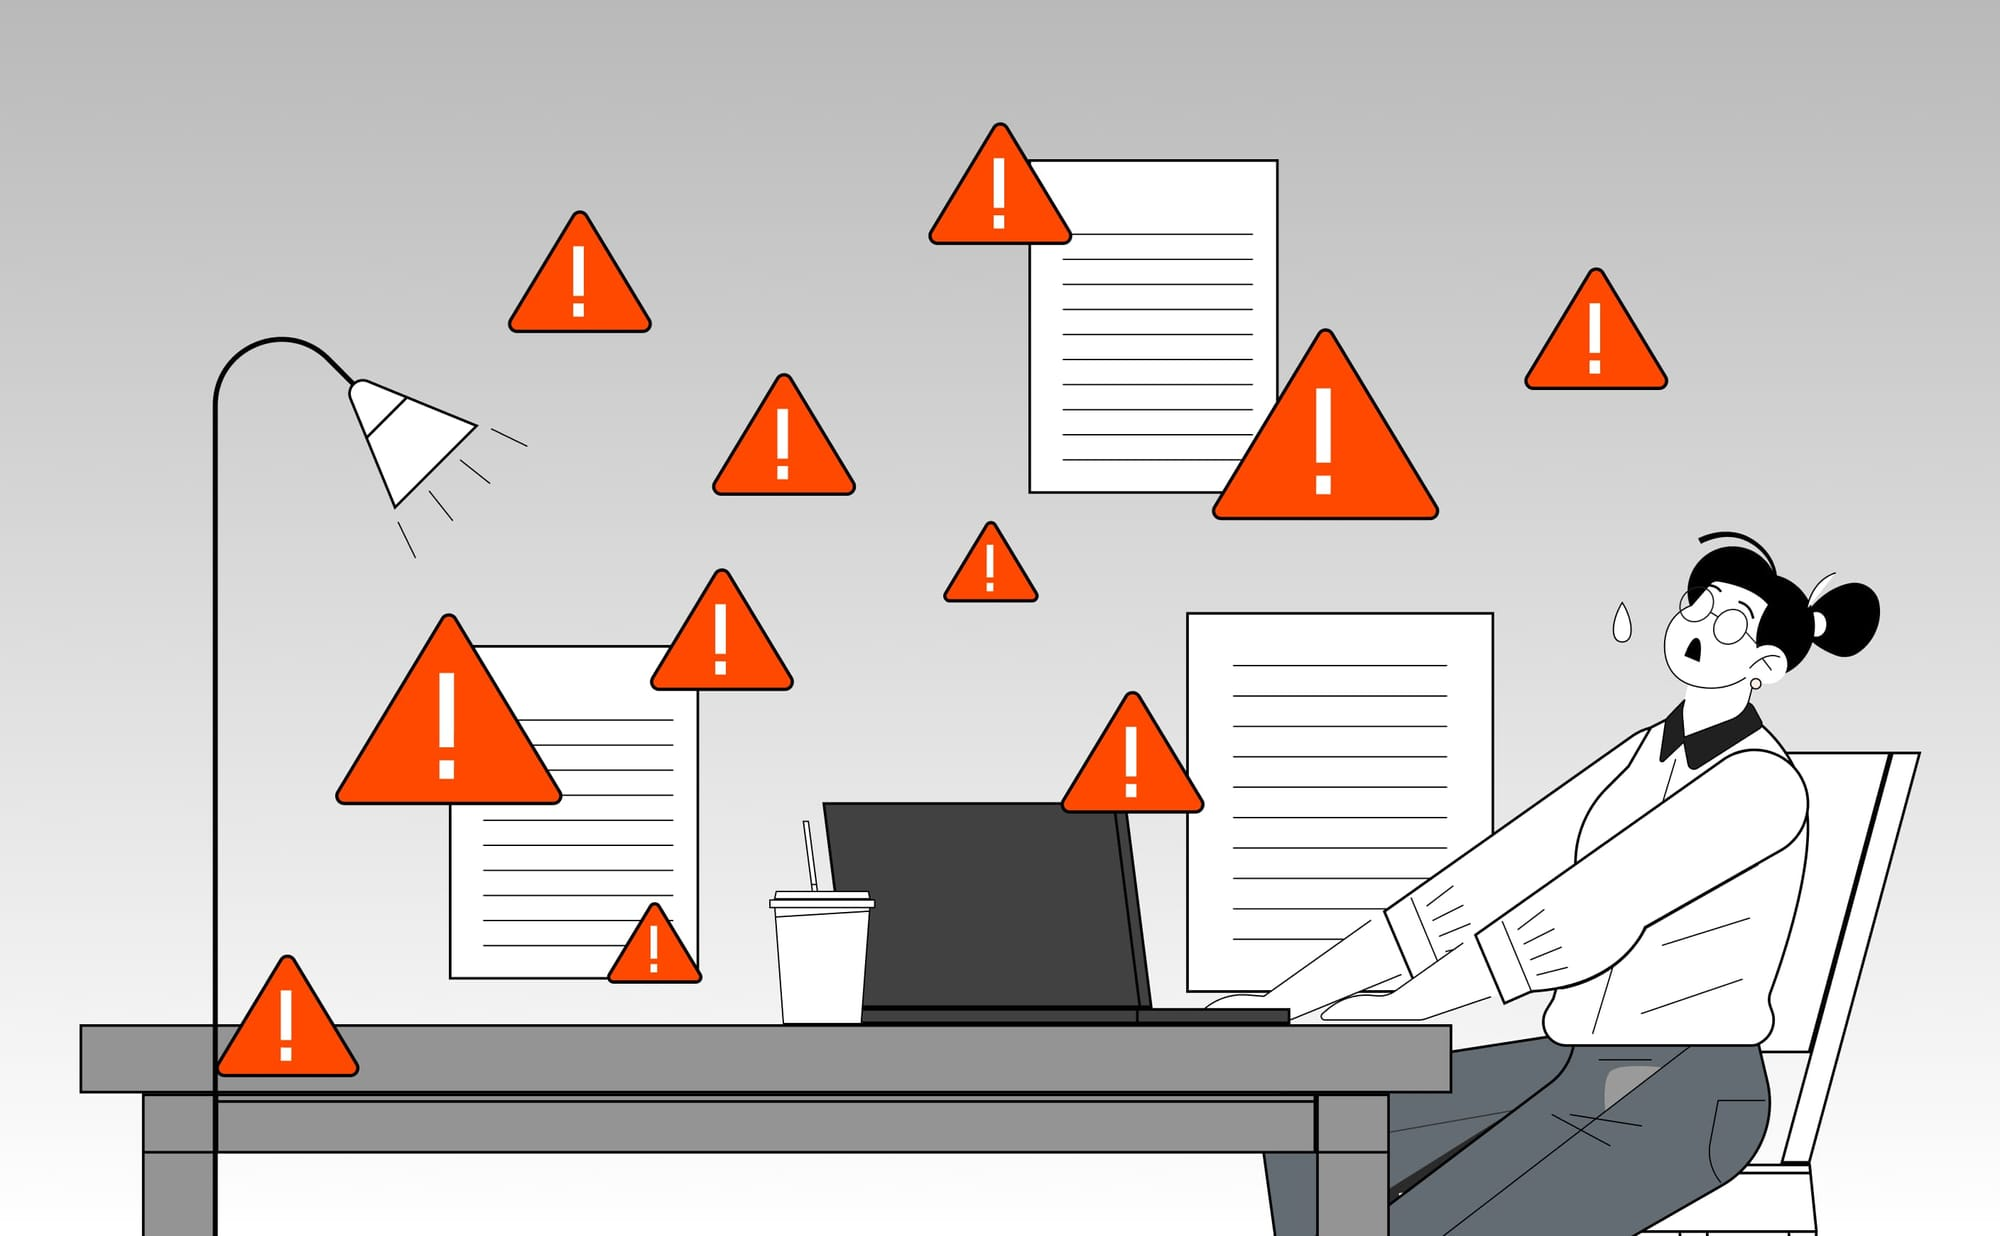
\includegraphics[width=1\linewidth]{alerts.png}
        \end{column}
        
        \begin{column}{0.32\textwidth}
            \begin{alertblock}{\centering Question}
            \centering
            \footnotesize \textbf{Comment doter les équipes techniques d'une plateforme intelligente \\--\\ \textit{capable d'assister la gestion des incidents} \\--\\ pour augmenter la productivité et réduire le MTTR ?}
            \end{alertblock}
        \end{column}
    \end{columns}
\end{frame}

\subsection{Objectifs}
\begin{frame}{Objectifs}
    \begin{figure}
        \centering
        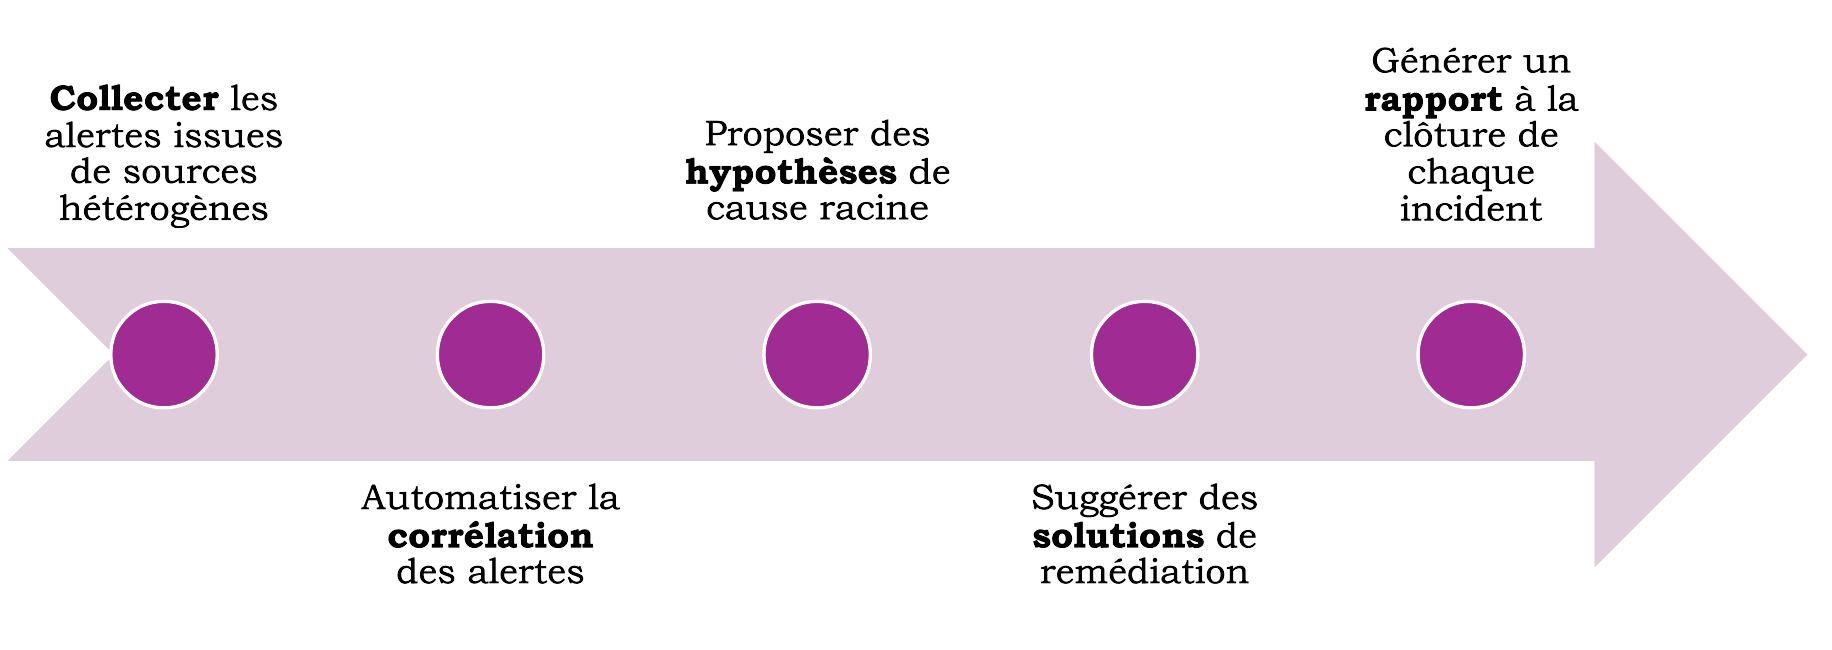
\includegraphics[width=1\linewidth]{obj.png}
    \end{figure}
\end{frame}

\section{Gestion des incidents}

\begin{frame}{Gestion des incidents}
    \begin{figure}
        \centering
        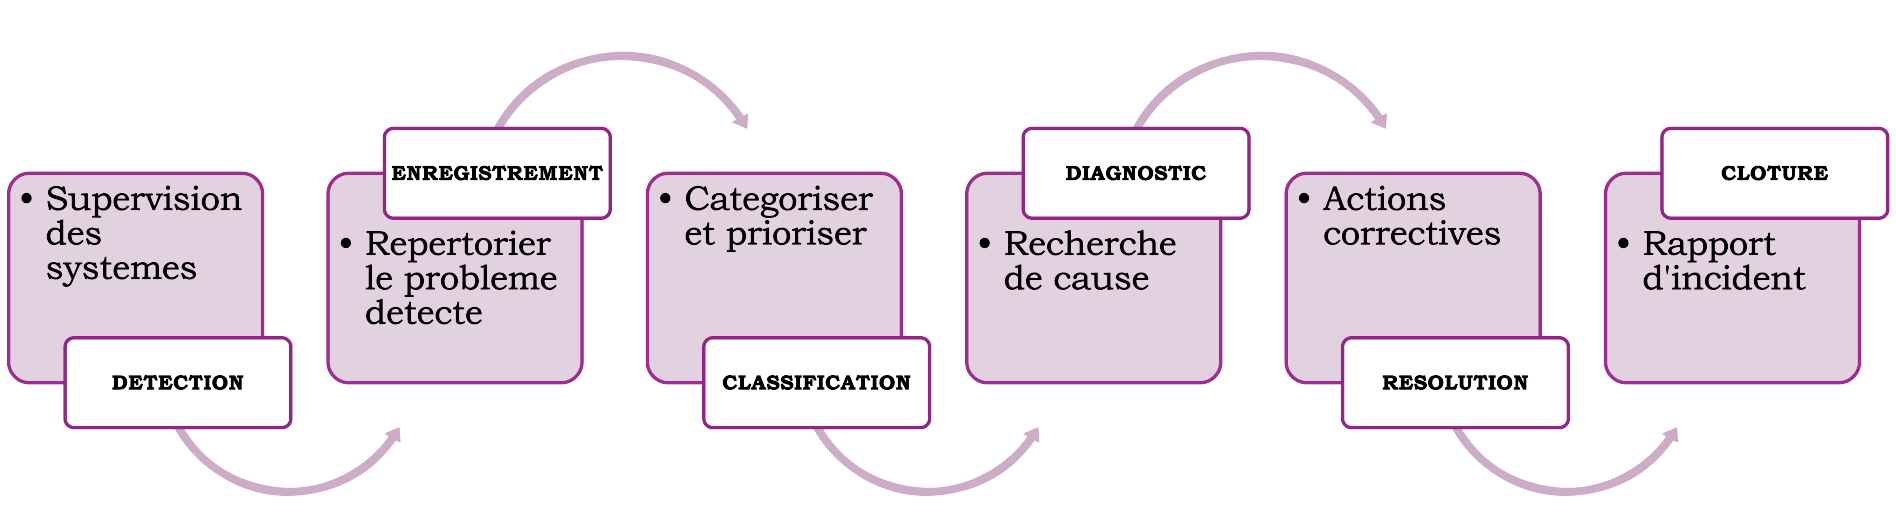
\includegraphics[width=1\linewidth]{process.png}
    \end{figure}
\end{frame}


\section{Conception}

\begin{frame}{Conception}
    % TODO : architecture globale, choix de conception
\end{frame}


\section{Réalisation}

\begin{frame}{Réalisation}
    % TODO : technologies, agents, intégration, captures de la plateforme
\end{frame}


\section{Résultat de test}

\begin{frame}{Résultat de test}
    % TODO : métriques des modèles, validation, démonstration
\end{frame}


\section{Conclusion et perspectives}

\begin{frame}{Conclusion et perspectives}
    % TODO : bilan, apports, perspectives d'amélioration
\end{frame}


\begin{frame}
    \maketitle
\end{frame}


\end{document}
